%//==============================--@--==============================//%
\clearpage
\subsection[4.3 Filtro adaptado]{$\rightarrow$ Filtro adaptado}
\label{subsec:matched-filter}

\begin{theo}[\underline{Matched filter}]{def:matched-filter}\label{def:matched-filter}
    $$
        h(t) \delequal \alpha s(T-t)\; \xrightleftharpoons[]{\mathcal{F}}\; H(f) \delequal \alpha S^*(f)e^{-j2\pi f T},\qquad \alpha \in \mathbb{R}
    $$

    \noindent $\pmb{\rightarrow}$ \textbf{Nota:} 
    $$
        r(t) \ast h(t)\biggr|_{t=T} = \int_{0}^{T} r(\tau)h(T-\tau) \,dt =  \int_{0}^{T} r(\tau)s(\tau) \,dt
    $$
    Então, um filtro adaptado\footnotemark[3] cujo \textit{output} é amostrado no instante $T$ extrai do sinal observado $r(t)$ as estatísticas suficientes para o problema da decisão.

    \vspace{-1em}
    \begin{figure}[H]
        \centering
        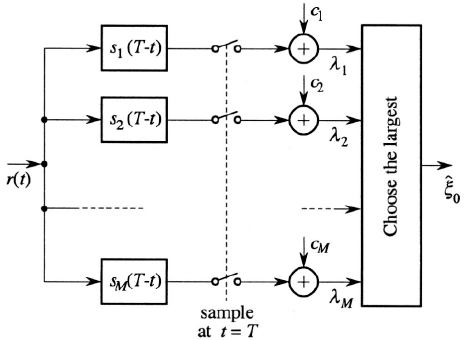
\includegraphics[width=0.5\linewidth]{img/digital/AWGN-transmission/detection-matched-filter.png} 
        \caption{Implementação do recetor ótimo coerente com filtros adaptados.\cite{Benedetto1999}} 
        \label{fig:detection-matched-filter} 
    \end{figure}
\end{theo}

\noindent Uma propriedade do filtro adaptado é que maximiza o SNR à saída. Quando a entrada do filtro é a soma do sinal $s(t)$ com ruído $n(t)$, no instante $t=T$, a sua saída será composta por dois termos: a primeira parte é respetiva ao sinal
$$
    \int_{-\infty}^{+\infty} H(f) S(f) e^{j2\pi f T} \,df,
$$
onde $H(f)$ representa a função de transferência do filtro; a segunda é respetiva à parte do ruído, uma VA gaussiana com média $\mu$ nula e variância dada por
$$
    \sigma^2 = \frac{N_0}{2}\int_{-\infty}^{+\infty} |H(f)|^2 \,df
$$
Se definirmos o SNR à saída do filtro como
$$
    \zeta^2 \delequal \dfrac{\displaystyle \left[ \int_{-\infty}^{+\infty} H(f) S(f) e^{j2\pi f T} \,df \right]^2}{\displaystyle \frac{N_0}{2}\, \int_{-\infty}^{+\infty} |H(f)|^2 \,df}
$$
É possível demostrar que tem o valor máximo para \underline{filtro adaptado}. Invocando a \hyperref[subsubsec:shwarz]{\underline{Desigualdade de Schwarz}} ($A = \alpha B^*$):
\vspace{-1em}
$$
    \rightarrow \left| \int_{\mathbb{R}} A\, B^* \right|^2 \leq \int_{\mathbb{R}} |A|^2\; \int_{\mathbb{R}} |B|^2
    \implies
    \zeta^2 \leq \frac{\displaystyle \cancel{\int_{\mathbb{R}} |H(f)|^2 \,df}\; \int_{\mathbb{R}} |S(f)|^2 \,df}{\displaystyle \frac{N_0}{2} \cancel{\int_{\mathbb{R}} |H(f)|^2 \,df}}
    = \frac{2 E_s}{N_0}
$$
\vspace{-1em}%adoro-te
$$
    \boxed{%
        \therefore \text{PSNR} \delequal \frac{2E_s}{N_0}
    }
$$
\footnotetext[3]{Para sinais pares, o filtro adaptado é uma réplica deslocada do pulso de entrada.}
%//==============================--@--==============================//%